\chapter{Návrh a realizácia konštrukcie dvojkolesového robota}

Proces návrhu hardvérového riešenia robota sme začali vytvorením zoznamu komponentov, potrebných pre realizáciu robota. Pri výbere komponentov a celkovom návrhu robota sme brali do úvahy požiadavku na modulárnosť robota. Pod pojmom modulárnosť rozumieme skonštruovanie robota tak, aby jednotlivé jeho časti mohli byť v prípade potreby jednoducho vymenené alebo upravené bez potreby väčších zásahov do celkovej konštrukcie. 

Robota sme teda rozdelili do viacerých funkčných celkov a pre každý z týchto celkov sme vytvorili samostatný zoznam komponentov. Vďaka tomuto postupu sme nielen znížili možnosť výberu nevyhovujúcich súčiastok, ale aj zabezpečili, že naše riešenie bude v prípade potreby škálovateľné a jednotlivé celky bude ľahké pozmeniť alebo doplniť o dodatočné časti. 


\underline{\textbf{Funkčné celky balansujúceho robota:}}
\begin{itemize}
\item napájanie
\item pohon
\item komunikácia
\item senzory
\item riadiaci mikropočítač
\end{itemize}

\section{Zoznam použitých komponentov}

V nasledujúcej časti práce opíšeme nami vybrané komponenty, ktoré boli využité pri konštrukcii robota. Zameriame sa hlavne na dôvod voľby daného komponentu, porovnáme špecifikácie použitých komponentov s našimi požiadavkami a zhodnotíme, ako dobre sa komponent hodí pre naše použitie.


\subsection{Napájanie}
Táto podkapitola obsahuje komponenty, ktoré poskytujú vhodné napájanie ostatným častiam robota.
\subsubsection{Batéria}
Pri výbere batérie sme sa snažili nájsť nabíjateľný model, ktorý by nám poskytol pri nízkej hmotnosti čo najvyššiu kapacitu, relatívne vysoký maximálny výstupný prúd a  výstupné napätie pohybujúce sa v rozmedzí 6 V až 12 V, ktoré je dostatočné pre väčšinu bežne dostupných jednosmerných motorov. Rozhodli sme sa pre 12V lítium-iónovú (Li-ion) batériu, využívajúcu tri 3,7 V články typu 18650. Kapacita batérie je 3300 mAh, maximálny okamžitý odoberaný prúd 5 A a maximálny pracovný prúd 3A. K nej priložený nabíjací adaptér je schopný dobíjať ju prúdom 1 A pri 12,6 V. Spolu s relatívne nízkou hmotnosťou 150g sa teda batéria z \figurename~\ref{fig:bateria} po každej stránke javí ako dobrá voľba. 

\begin{figure}[h]
\centering
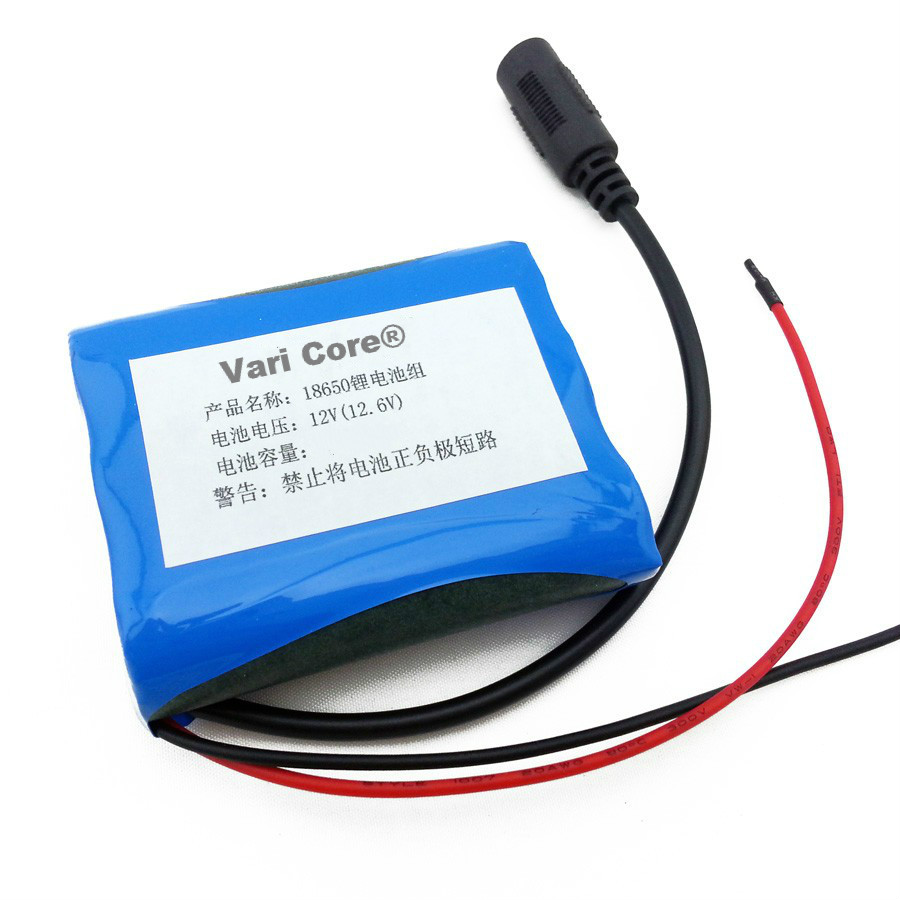
\includegraphics[width = 6cm]{bateria}
\caption{Li-ion batéria\cite{VariCore}}
\label{fig:bateria}
\end{figure}


\bgroup
\def\arraystretch{1.8}
\begin{table}[h]
\centering
\begin{tabular}{|c|c|c|c|c|}
\hline
Výs. napätie [V] & Max. výs. prúd [A] & Pracovný prúd [A]  & Hmotnosť [kg]&Technológia\\
\hline
 12& 5 & 3  & 0.15& Li-ion \\
\hline
\end{tabular}
\caption{Parametre batérie}
\label{tab:bateria}
\end{table}
\egroup

\subsubsection{Napäťový regulátor pre logické obvody}
Jedným z možných riešení pre napájanie logických obvodov robota, bolo použitie sekundárnej $5~V$ batérie. Toto riešenie sa ale nejavilo v tomto prípade ako optimálne, keďže druhá batéria by zaberala miesto a vyžadovala si samostatný napájací adaptér. Rozhodli sme sa preto využiť už zabudovanú $12~V$ batériu napájajúcu motory v kombinácii s paralelne pripojeným napäťovým regulátorom. 

Rozhodovali sme sa medzi rozšíreným integrovaným obvodom L7805CV, ktorý predstavuje $5~V$ lineárny napäťový regulátor a modulom MP1584. Modul MP1584\figurename~\ref{fig:napRegulator} je spínaným napäťovým regulátorom a obsahuje integrovaný obvod LM2596\cite{LM2596} . Vďaka vlastnostiam LM2596, medzi ktoré patrí vysoká účinnosť (až 92\%), malé kolísanie výstupného napätia a možnosť riadenia výstupného napätia od $4~V$ – $35~V$ sme sa nakoniec rozhodli použiť ako napäťový regulátor modul MP1584.

\begin{figure}[h!]
\centering
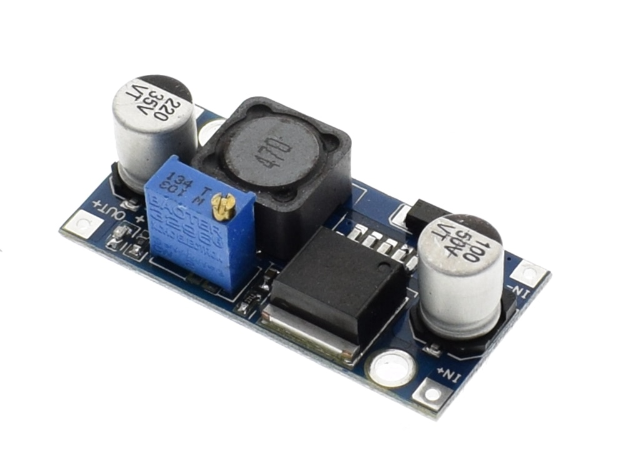
\includegraphics[width=6cm]{napRegulator}
\caption{Modul MP1584\cite{MP1584}}
\label{fig:napRegulator}
\end{figure}

\subsection{Pohon}
Pre samotný pohyb robota je potrebné správne zvoliť vhodný typ motora a obvodu, ktorý bude môcť podľa pokynov mikropočítača dané motory ovládať. V našom prípade sme vyberali motory, ktoré budú poháňať kolesá robota, aj servomotor umožňujúci robotu pohybovať sa aj po naklonených plošinách.

\subsubsection{Motory}
V prípade motorov sme mali na výber z viacerých možností, pričom hlavným kritériom bolo, že sa musí ísť o jednosmerné motory primeranej veľkosti. Aj tak sme ale mohli voliť medzi bezkomutátorovým, krokovým a motorom s permanentnými magnetmi. Po úvahe a prieskume bežne dostupných motorov sme sa rozhodli pre klasický motor s permanentnými magnetmi využívajúci komutátor. Tento motor má niekoľko nevýhod, ako sú napríklad malá presnosť v porovnaní s krokovým motorom a menší moment spolu s rýchlejším opotrebením v porovnaní s motorom bez komutátora. Napriek týmto nevýhodám sú tieto motory ale vhodné pre naše účely, lebo sú lacné, jednoduché na ovládanie a dostupné v mnohých konfiguráciách. 

Po zvážení sme sa rozhodli pre $12~V$ motory typu GM25-370CA, s integrovanou prevodovkou 1:21 a zabudovanými dvojkanálovými enkodérmi, ktoré nám umožnia odometrickým meraním sledovať zmenu pozície kolies napojených na motor. Dokumentácia uvádza max. rýchlosť nezaťaženého motora ako 280 \ac{RPM} (otáčok za minútu), pričom túto max. rýchlosť potvrdili aj naše merania. Výhodou týchto motorov je aj to, že je ich možné dostať v konfigurácii priamo určenej pre robotické platformy podobné našej spolu s kolesami a kovovým podvozkom. Nevýhodou týchto motorov je relatívne veľká vôľa kolies a nízke rozlíšenie integrovaných enkodérov.  

\begin{figure}[h!]
\centering
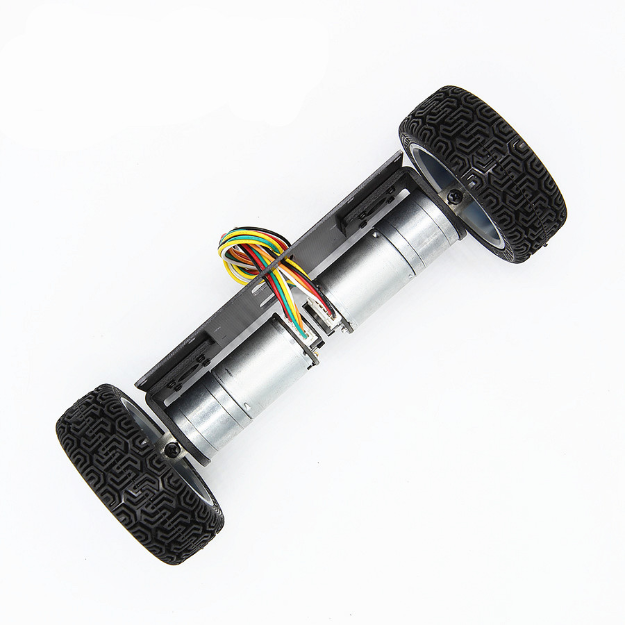
\includegraphics[width=6cm]{motorPlatforma}
\caption{Platforma s motormi\cite{wheelBase}}
\label{fig:motorPlatforma}
\end{figure}

\subsubsection{H-mostík}
Keďže mikropočítač nie je bez externej elektroniky schopný sám dodávať do motora potrebný výkon, je potrebné spolu s ním použiť tzv. H-mostík. Ten predstavuje principiálne iba štyri elektricky ovládané spínače \figurename~\ref{fig:h_bridge_scheme}, ktoré podľa svojej konfigurácie menia smer toku prúdu motorom - teda smer otáčania motora. Naše požiadavky na H-mostík boli: vysoká účinnosť, jednoduché prepojenie s mikropočítačom, galvanicky oddelené vstupy mikropočítača a schopnosť dodať motorom dostatočný výkon (výrobca uvádza maximálny odber $3,5~A$ na motor). 

Našou voľbou bol dvojitý H-mostík kompatibilný s integrovaným obvodom L298, ktorý spĺňa všetky naše požiadavky a je schopný dlhodobo dodávať do motorov až $7~A$ pri napätí $12~V$. Tento obvod je možné prepojiť s mikropočítačom pomocou šiestich vstupov, pričom štyri slúžia na výber konfigurácie spínačov a dva prijímajú \ac{PWM} signál, ovládajúci pripojenie batérie na vstup motorov. Je teda možné jednoducho meniť striedu jednotlivých motorov a tým aj ich rýchlosť. Pre svoju správnu činnosť vyžaduje tento H-mostík napájanie $5~V$, to nám poskytne nami použitý napäťový regulátor. 

\begin{figure}
\centering
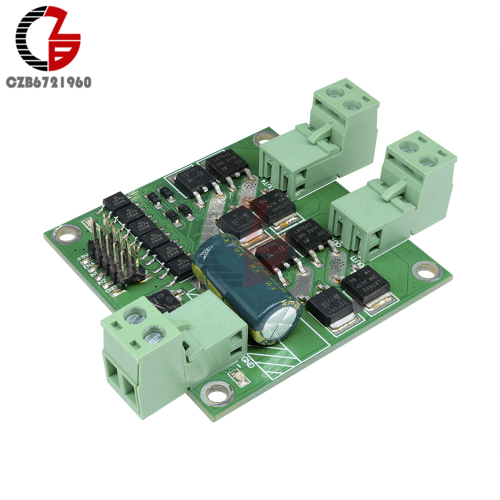
\includegraphics[width=6cm]{hMostik}
\caption{H-mostík komaptibilný s L298\cite{hBridge}}
\label{fig:hMostik}
\end{figure}

\subsubsection{Servomotor}
Jednou z dodatočných požiadaviek na náš balansujúci robot bolo, aby sa šasi robota mohlo pohybovať do strán nezávisle od platformy s kolesami. Táto funkcionalita nám v praxi poskytne vyššiu kontrolu nad robotom v zákrutách, na naklonených plošinách a do určitej miery zníži pravdepodobnosť pádu v prípade pôsobenia silou na bočnú časť robota.

Za optimálne riešenie sme považovali jednoduché servo HJ S3315D určené prevažne na modelárske účely. Toto servo dodatočne taktiež spojí platformu s kolesami a šasi robota, ktorým bude takto možné v prípade potreby hýbať o presne určené uhly. V takejto konfigurácii  obmedzenie pohybu serva v rozmedzí -90º až 90º nepredstavuje problém.


\begin{figure}[h]
\centering
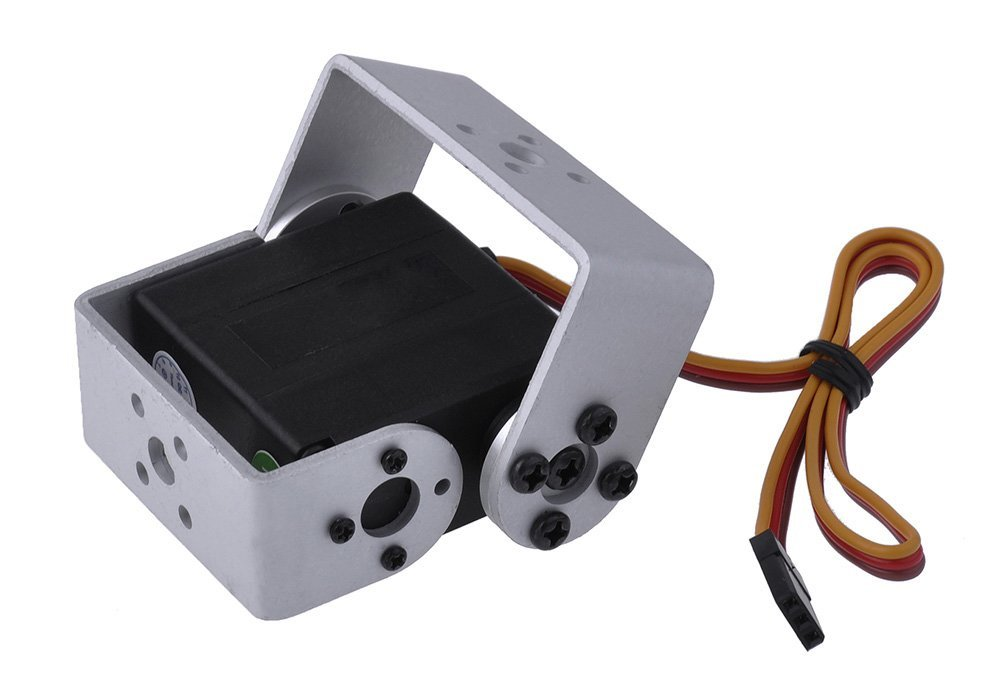
\includegraphics[width=8cm]{servoMotor}
\caption{Servo motor HJ S3315D\cite{servoMotor}}
\label{fig:servoMotor}
\end{figure}
\subsection{Komunikácia - Bluetooth modul}
Okrem neriadeného balansovania na mieste musí byť robot tiež schopný prijímať od operátora na diaľku príkazy a pohybovať sa v priestore podľa pokynov. Taktiež je nutné, aby bol robot v prípade požiadania operátora schopný poskytnúť základné informácie o svojom stave, napr. úroveň nabitia batérie, priemernú rýchlosť pohybu za určitý časový interval, okamžitý uhol náklonu,… Tieto informácie musí byť robot schopný poskytnúť s čo najmenším oneskorením, bezdrôtovo a minimálne na vzdialenosť 10 metrov.  
\begin{figure}[h!]
\centering
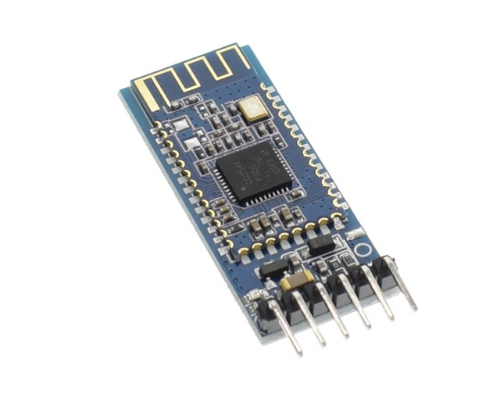
\includegraphics[width=8cm]{bluetoothModul}
\caption{HC05-Bluetooth modul\cite{bluetoothModule}}
\label{fig:bluetoothModul}
\end{figure}
Rozhodli sme sa použiť Bluetooth vysielač/prijímač HC-05. Tento modul sa vyznačuje integrovanou anténou, nízkym operačným napätím (min. $1.3~V$) a je schopný prijímať aj odosielať dáta pomocou štandardného rozhrania \ac{UART} (Universal Asynchronous Reciever-Transmitter). Dosah tohto modulu je na stránke predajcu uvádzaný až do $10~m$.

Využitím tohoto modulu v robotovi aj v ovládači, ktorým ho budeme ovládať zabezpečíme možnosť odosielať jednoduché povely na riadenie robota aj prijímať komplexné dáta o jeho aktuálnom stave.

\subsection{Senzory}
Pod senzormi rozumieme všetky časti robota, ktoré mu umožňujú získavať informácie o jeho okolitom prostredí, ale aj o jeho vlastnom stave. Pre naše účely je nevyhnutné presne merať uhol náklonu robota a rýchlosť pohybu motorov.

\subsubsection{MPU 6050}
Pre úspešné balansovanie robota je potrebná relatívne vysoká presnosť merania uhla náklonu robota. Ak by sme postupovali využitím akcelerometra, prístroja určujúceho uhol náklonu podľa pôsobenia gravitačného zrýchlenia, nebolo by toto meranie dosť presné, keďže pri rýchlych zmenách polohy je akcelerometer ovplyvnený zrýchlením robota a vibráciami. Výhodou merania z akcelerometra je však veľmi vysoká presnosť merania v ustálenom stave. 

Na druhú stranu z dát získaných pomocou gyroskopu, prístroja merajúceho uhlovú rýchlosť, sme schopní určiť zmenu uhla náklonu robota za čas $dt$ integráciou nameraných hodnôt. Tieto merania zmeny uhla sú presné aj pri rýchlych pohyboch robota. Nevýhodou použitia gyroskopu ale je, že aj tá najmenšia chyba pri každom meraní a integrovaní sa započíta do výsledku a po niekoľkých stovkách meraní je už chyba merania uhla značná – tomuto javu sa hovorí gyroskopický drift. 
\begin{figure}[h]
\centering
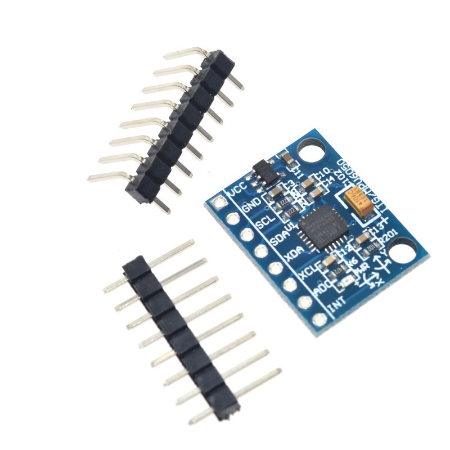
\includegraphics[width=8cm]{MPU}
\caption{Modul GY-521\cite{GY-521pic}}
\label{fig:MPU}
\end{figure}
Riešenie problému merania uhla u pohybujúceho sa robota predstavuje kombinácia nameraných hodnôt z akcelerometra a gyroskopu, pomocou komplementárneho filtra. Na toto využite sa hodí modul GY-521 obsahujúci senzor MPU 6050\cite{MPU6050datasheet}, ktorý v sebe kombinuje trojosový akcelerometer a gyroskop. Modul je schopný komunikovať s mikropočítačom pomocou rozhrania I2C maximálnou rýchlosťou 400kHz a obsahuje taktiež integrovaný teplomer a DMP (Digital Motion Processor).Ten je schopný priamo uskutočniť analýzu nameraných dát, čím sa znížia požiadavky na výpočtový čas mikropočítača.



\subsection{Riadiaci počítač - Arduino MEGA}
Vďaka skúsenostiam s programovaním mikropočítačov spoločnosti Microchip-Atmel sme sa pri výbere mikropočítača rozhodovali medzi mikropočítačmi rodiny ATMEGA. Do úvahy prichádzali hlavne ATMEGA328P\cite{ATMEGA328} a ATMEGA2560\cite{ATMEGA2560}, ktorých výpočtové možnosti a zabudované periférie postačovali našim požiadavkám. Jednou zo zvažovaných možností bolo navrhnutie a skonštruovanie obvodu so zabudovaným mikropočítačom, ktorý by priamo zodpovedal požiadavkám našej aplikácie. Toto riešenie sme ale nakoniec po úvahe zavrhli, keďže by bolo časovo náročné a nespadalo by do koncepcie modularity – takto navrhnutý obvod by v prípade poruchy bol náročný na nahradenie a bolo by veľmi náročné upraviť ho pri zmene požiadaviek na robota.

Rozhodli sme sa teda využiť rozšírenú otvorenú vývojovú platformu Arduino, ktorá vo všeobecnosti slúži na vývoj prototypov a testovanie kódu. Našou voľbou bolo Arduino MEGA \figurename~\ref{fig:arduinoMega}, využívajúce mikropočítač ATMEGA2560. Táto vývojová doska má zabudovaný programovací port USB typu B (ktorý sme zamenili na micro USB), napäťový regulátor na 5V a 3.3V, 16 MHz oscilátor (zdroj hodinového signálu pre mikropočítač) a na rozdiel od lacnejšieho Arduino Uno má až 53 GPIO (General Purpose Input Output) pinov, 16 pinov podporujúcich ADC (prevod analógového signálu na jeho digitálnu reprezentáciu) a 6 pinov podporujúcich niekoľko režimov prerušení.

\begin{figure}[h]
\centering
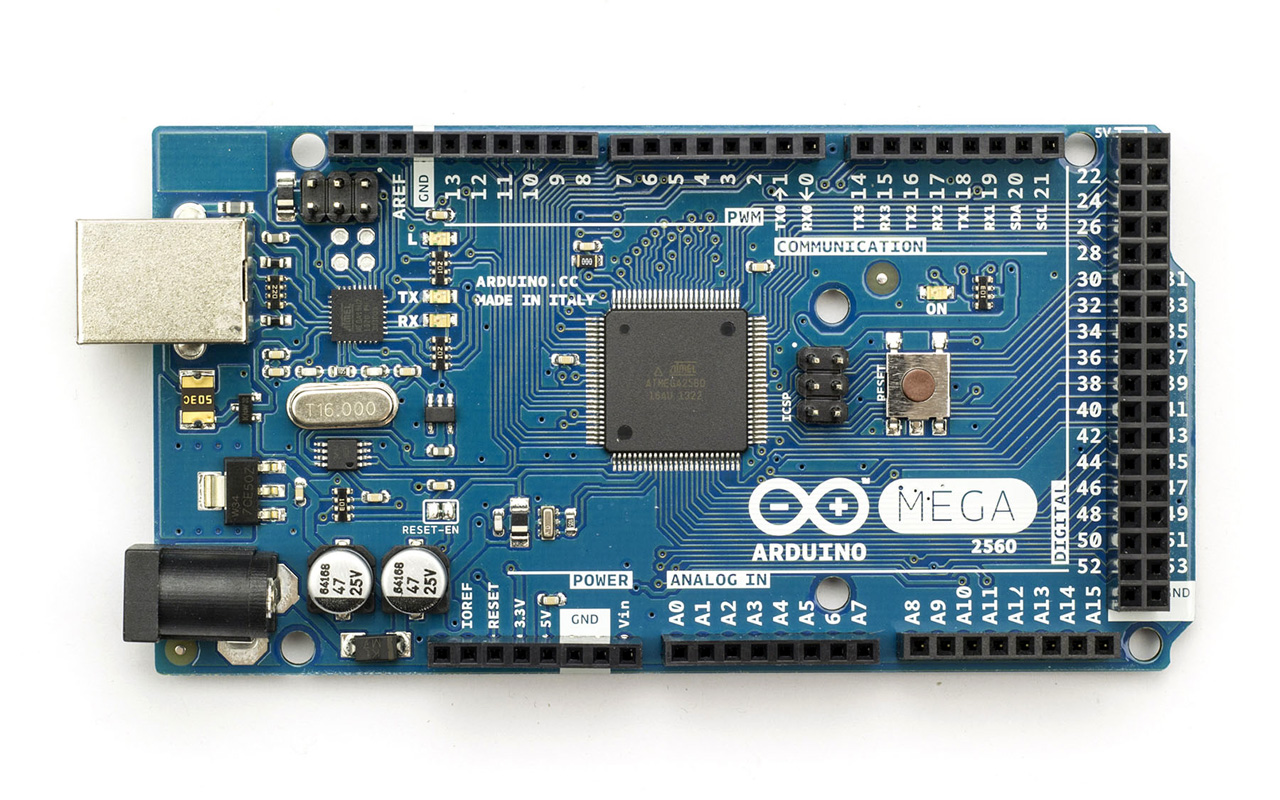
\includegraphics[width=8cm]{arduinoMega}
\caption{Arduino Mega\cite{arduinoMEGA}}
\label{fig:arduinoMega}
\end{figure}

Samotný mikropočítač má viacero časovačov, ktoré umožňujú napr. merať časové intervaly a generovať PWM signál, ale taktiež 4 páry RX, TX pinov slúžiacich na komunikáciu pomocou UART protokolu. Ako ďalšie možnosti komunikácie je možné využiť aj I2C a SPI protokoly. Programovanie dosky Arduino MEGA je možné cez USB rozhranie, napr. pomocou programu ArduinoIDE, AtmelStudio alebo Eclipse. Našou voľbou bolo využitie všestranného editora Eclipse, v kombinácii s pluginom umožňujúcim jednoduchú prácu s mnohými produktami Microchip-Atmel.



\section{Návrh a výroba šasi robota}
Pri výrobe šasi robota sme sa rozhodli použiť technológiu 3D tlače. S jej použitím sme boli schopný vytvoriť pevné a ľahké šasi, ktoré presne zodpovedalo našim požiadavkám. Pred samotnou tlačou sme ale museli navrhnúť model v CAD programe tak, aby bolo nielen jednoduché ho vytlačiť, ale aj aby bolo schopné odolať nárazom a ochrániť tak elektroniku vo vnútri. Pri návrhu sme použili software Fusion 360, ktorý je pre študentov dostupný zdarma na stránke firmy \href{https://www.autodesk.com/products/fusion-360/overview}{Autodesk}.

Program Fusion 360 podporuje ako návrh a export modelov do viacerých bežne používaných formátov, tak aj analýzu vlastností modelu, simuláciu jeho správania pri záťaži, nástroje na vizualizáciu, animáciu a mnoho ďalších užitočných funkcií.

Nami vytvorené šasi  sa skladá z dvoch častí a to veka a miskovitého tela, v ktorom sú uložené komponenty. Po naštudovaní prác, ktoré už boli na tému návrhu dvojkolesového balansujúceho robota napísané, sme zvolili pre celé šasi klinovitý tvar s úzkou podstavou a širokých vrchom. Tento tvar nám umožní jednoduché napojenie servomotora na spodnú časť robota a osadenie batérie blízko k hornej časti robota. V takomto usporiadaní dosiahneme relatívne vysoko umiestnené ťažisko, čo následne zjednoduší stabilizovanie robota. Šasi taktiež obsahuje otvory na kabeláž od motorov, dve LED diódy indikujúce stav robota, spínač napájania a prístup k portu micro USB, vďaka ktorému je možné robota programovať bez nutnosti demontáže veka.

Tlač prebehla po vytvorení gcode súboru v nástroji Cura na tlačiarni Creality CR-10s. Na tlač bol použitý materiál PLA (Polyactic Acid), ktorý sa vyznačuje nízkou tepelnou rozťažnosťou pri chladnutí, nízkou cenou a jednoduchou tlačou. 

\begin{figure}
\centering
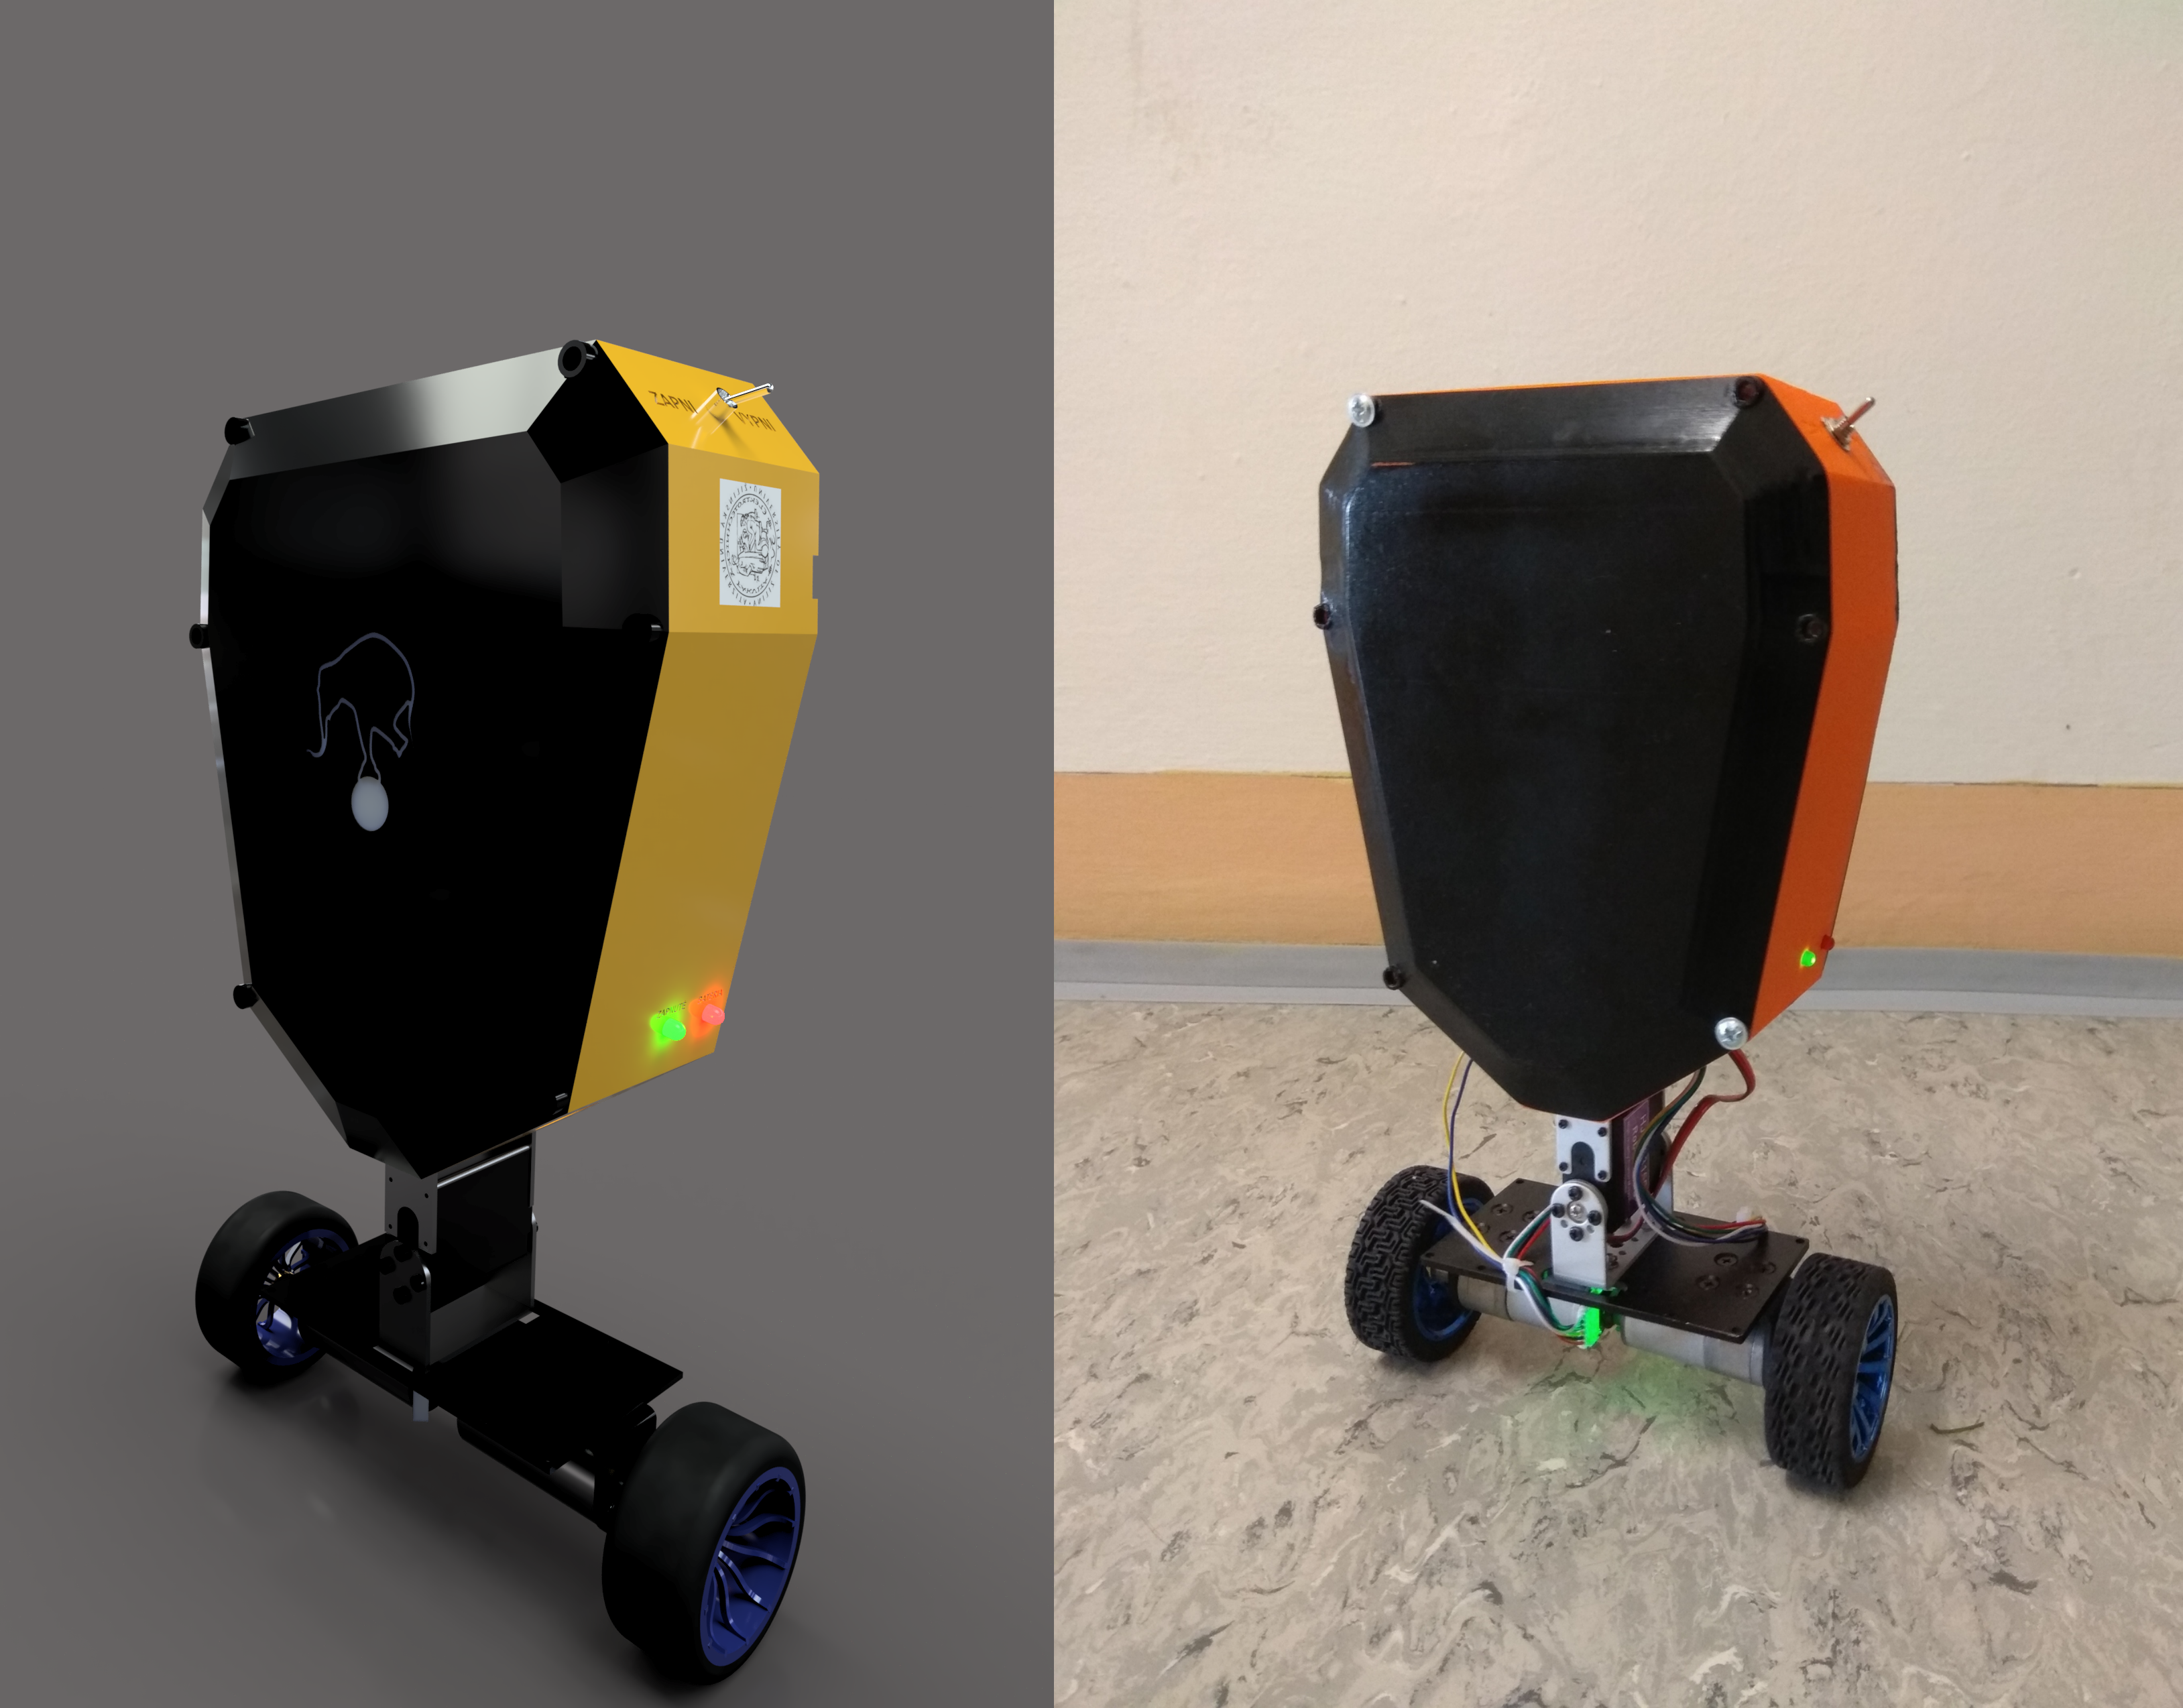
\includegraphics[width=14cm]{robotComp}
\caption{Porovnanie modelu a reálnej podoby robota}
\label{fig:robotComp}
\end{figure}

Samotná tlač trvala približne až 50 hodín, kvôli požiadavke na relatívne vysokú presnosť (a teda malú výšku jednotlivých vrstiev), pričom sa pri nej spotrebovalo približne $0,5~kg$ PLA. Po vytlačení, osadení komponentov a nalakovaní sa nami vytvorený model výzorom blížil k jeho počítačovo vygenerovanej podobe viď. \figurename~\ref{fig:robotComp}. Po kontrole môžeme tiež konštatovať, že vnútorné a vonkajšie rozmery oboch dielov presne zodpovedali nášmu návrhu.

Pri tlači sa vyskytli menšie chyby, ktoré spôsobili artefakty na veku robota v podobe pruhov spôsobených krycou páskou na podstave tlačiarne. Ako problematické sa ukázalo taktiež vytlačenie tela, na ktorého povrchu boli po vytlačení viditeľné chyby v podobe nezaplnených miest a príliš zaoblených hrán. Tie mohli byť spôsobené nesprávnym nastavením parametrov v programe Cura, privysokou teplotou vyhrievanej podstavy tlačiarne alebo príliš priľnavou podstavou. 

Výsledné výtlačky boli ale použiteľné, keďže vyššie opísané chyby boli čisto estetického charakteru. Ako závažnejším problémom sa ukázala realizácia kabeláže. Napriek dostatku miesta bolo po zapojení všetkých komponentov náročné sa v kabeláži vyznať, čo by mohlo spôsobiť problémy pri dodatočnej údržbe. 

Na vyriešenie tohto problému sme navrhli a dali vyhotoviť tzv. shield. Tento shield je doska plošných spojov, ktorá svojim vyhotovením predstavuje nadstavbu Arduina. Takýto shield je možné jednoducho pripojiť k Arduinu a jeho výhodou je tiež, že môže obsahovať označené terminály, umožňujúce bezpečné pripojenie komponentov k Arduinu. 

\begin{figure}[h]
\centering
\begin{minipage}[b]{0.48\textwidth}
\centering
\includegraphics[width=\textwidth]{robotInsideFoto}
\caption{Pred osadením shieldu}
\label{fig:robot_no_shield}
\end{minipage}\quad
\begin{minipage}[b]{0.48\textwidth}
\centering
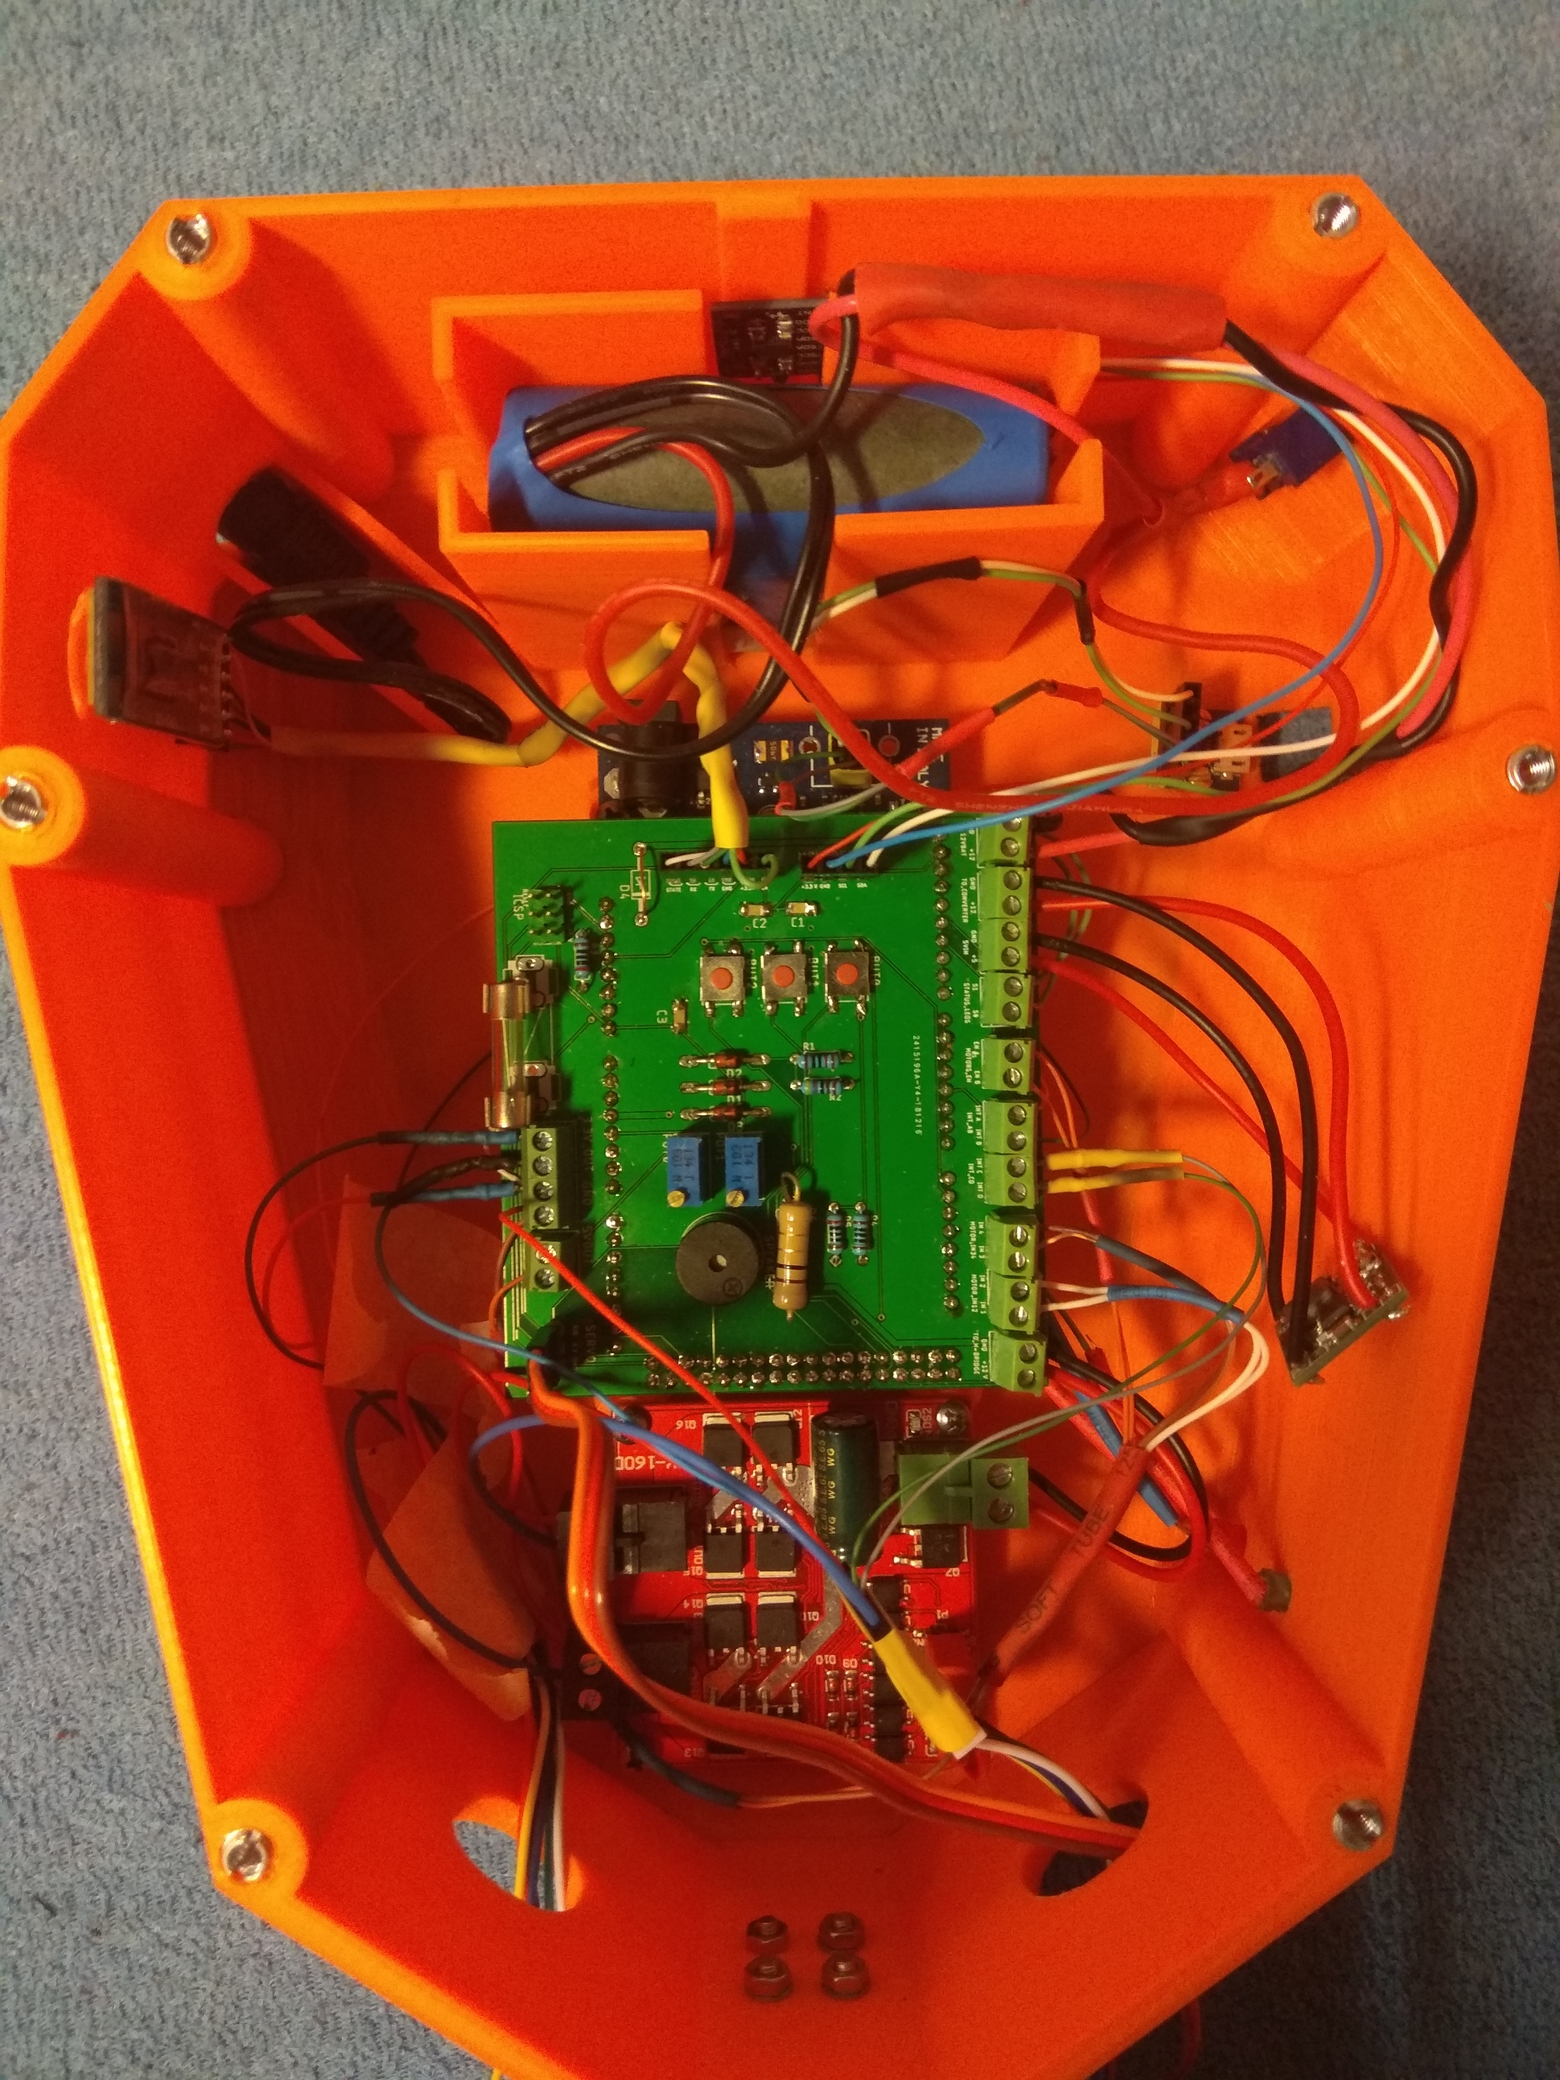
\includegraphics[width=\textwidth]{shield}
\caption{Po osadení shieldu}
\label{fig:robot_shield}
\end{minipage}
\label{fig:comparison}
\end{figure}

Návrh tejto dosky plošných spojov sme uskutočnili v bezplatnej verzii nástroja Eagle. Tá umožňuje návrh elektrických schém aj PCB (Printed Circuit Board) a generovanie gerber súborov, ktoré obsahujú informácie pre výrobcu. Ukážka takto vytvorenej dosky je v prílohe \figurename~\ref{fig:neosadenyShield}, pričom pri jej tvorbe sme vychádzali zo schémy na \figurename~\ref{fig:schemaShield}. 

Zo schémy je zjavné, že nami vytvorený obvod obsahuje okrem vstupno/výstupných terminálov aj dodatočnú ochranu vstupov proti prepätiu. Táto je realizovaná formou Zenerových diód s hodnotou prierazného napätia 5 V, zapojených v závernom smere. Napriek tomu, že mikropočítač ATmega 2560 obsahuje zabudované diódy, ktoré vedia vstupy ochrániť proti krátkodobému prepätiu, externé zenerove diódy prejdú do vodivého stavu skôr a zabránia tak prípadnému poškodeniu mikropočítača prepätím. 

Medzi ďalšie ochranné prvky, ktoré sme implementovali, patrí Shottkyho dióda zapojená do série s batériou, ktorá zabráni poškodeniu komponentov v prípade nesprávneho pripojenia batérie. Podobným spôsobom zapojená tavná poistka ochráni batériu pred možným skratom v obvode.  Keďže bluetooth modul, ktorý sme zvolili pre realizáciu komunikácie, pracuje s logickými úrovňami od $0 V$ do $3,3 V$, ale Arduino výstupy pracujú s $5 V$, pripojili sme RX vstup modulu k mikropočítaču cez napäťový delič. 

Doska plošných spojov obsahuje aj dva potenciometre, tri spínače a reproduktor. Potenciometre a spínače budú v prípade potreby slúžiť na jemnú kalibráciu alebo manuálne zadávanie jednoduchých povelov. Reproduktor so zabudovaným oscilačným obvodom slúži ako hlásič, napr. v prípade prebiehajúcej kalibrácie. Kompletná schéma nami navrhnutého shieldu je v prílohe na \figurename~\ref{fig:schemaShield}. Porovnanie vnútra robota pred a po osadení shieldu je na \figurename~\ref{fig:robot_no_shield}, \figurename~\ref{fig:robot_shield}.

\section{Výsledky montáže a zhodnotenie návrhu}
Nami navrhnutý dizajn robota sa v praxi ukázal ako veľmi jednoduchý na skonštruovanie. Po vytlačení šasi robota na 3D tlačiarni stačilo len spojiť skrutkami servo, šasi a podvozok robota a následne zrealizovať kabeláž podľa schémy \figurename~\ref{fig:schemaShield}.Finálny vzhľad robota po zmontovaní je na \figurename~\ref{fig:robot_front} \figurename~\ref{fig:robot_side}. Do vnútra šasi robota sme bez problémov nainštalovali všetky potrebné komponenty a ponechali dostatok voľného miesta na prípadné neskoršie úpravy robota.   

\begin{figure}[h]
\centering
\begin{minipage}[b]{0.48\textwidth}
\centering
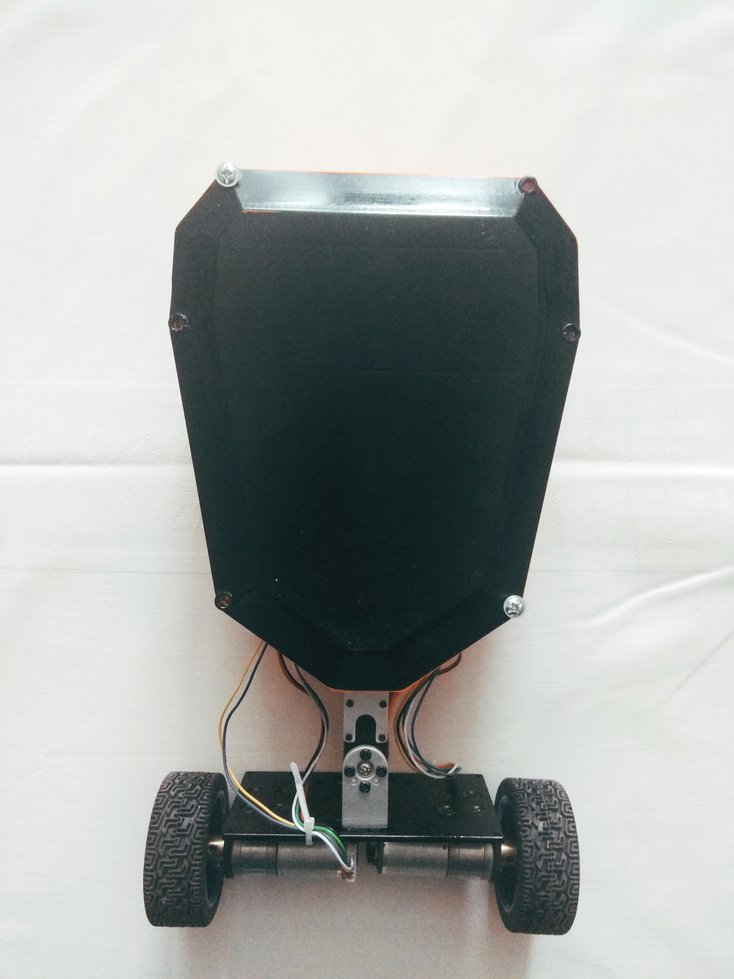
\includegraphics[width=\textwidth]{front_robot}
\caption{Robot spredu}
\label{fig:robot_front}
\end{minipage}\quad
\begin{minipage}[b]{0.48\textwidth}
\centering
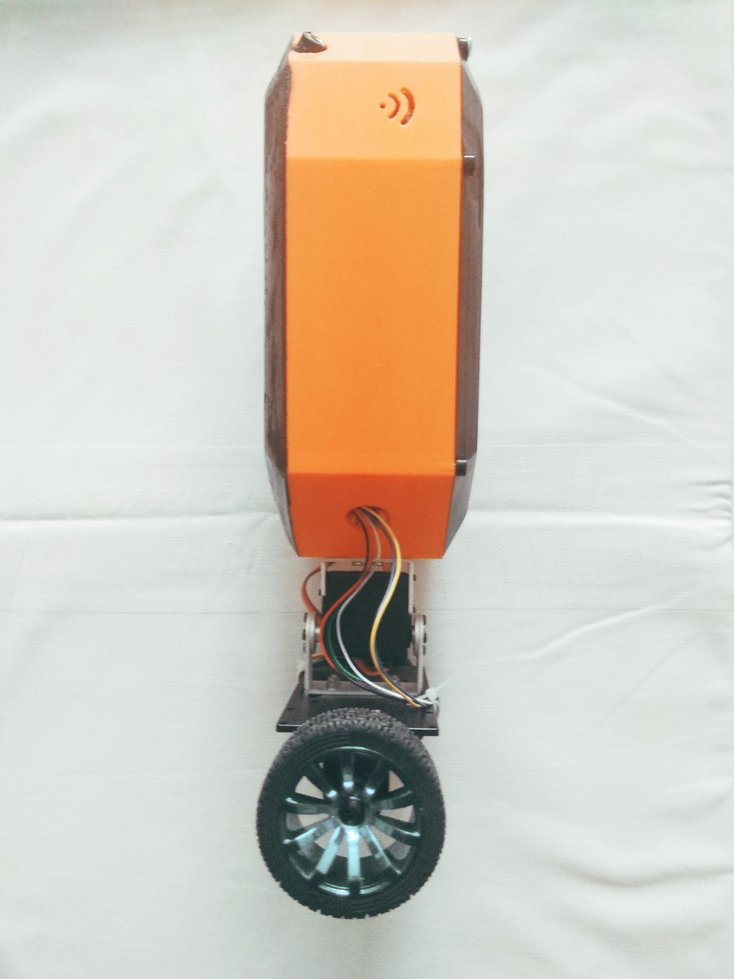
\includegraphics[width=\textwidth]{side_robot}
\caption{Robot zboku}
\label{fig:robot_side}
\end{minipage}
\end{figure}

Pri motáži sme ale identifikovali niekoľko nedostatkov nášho návrhu. Jedným z nich bolo nevhodné umiestnenie senzora MPU6050 priamo nad batériou, čím sme značne limitovali možnosti prístupu k senzoru po montáži. Samotný priestor pre osadenie batérie bol pôvodne navrhnutý bez veka, ktoré by zabránilo batérií v pohybe pri činnosti robota. Navrhnúť vhodné veko sa ale ukázalo ako značne náročné. Dôsledkom toho bolo, že batéria musela byť ukotvená použitím lepidla, čo nie je najvhodnejšie riešenie, pretože značne komplikuje prípadnú výmenu batérie za iný model.    

\section{Návrh a výroba ovládača robota}

Pri návrhu ovládača robota sme postupovali podobným spôsobom ako pri návrhu šasi. Rovnako ako pri šasi aj tu bol na návrh ovládača použitý nástroj Fusion 360 a technológia 3D tlače. Takto navrhnutý ovládač obsahuje dvojosový analógový joystick, ktorý riadi pohyb robota a umožňuje používateľovi pohyb v menu nastavení. Informácie získava používateľ zo zabudovaného 1,8 palcového farebného TFT displeja. Orientáciu v menu zjednodušujú dve zabudované tlačidlá.

\begin{figure}[h]
\centering
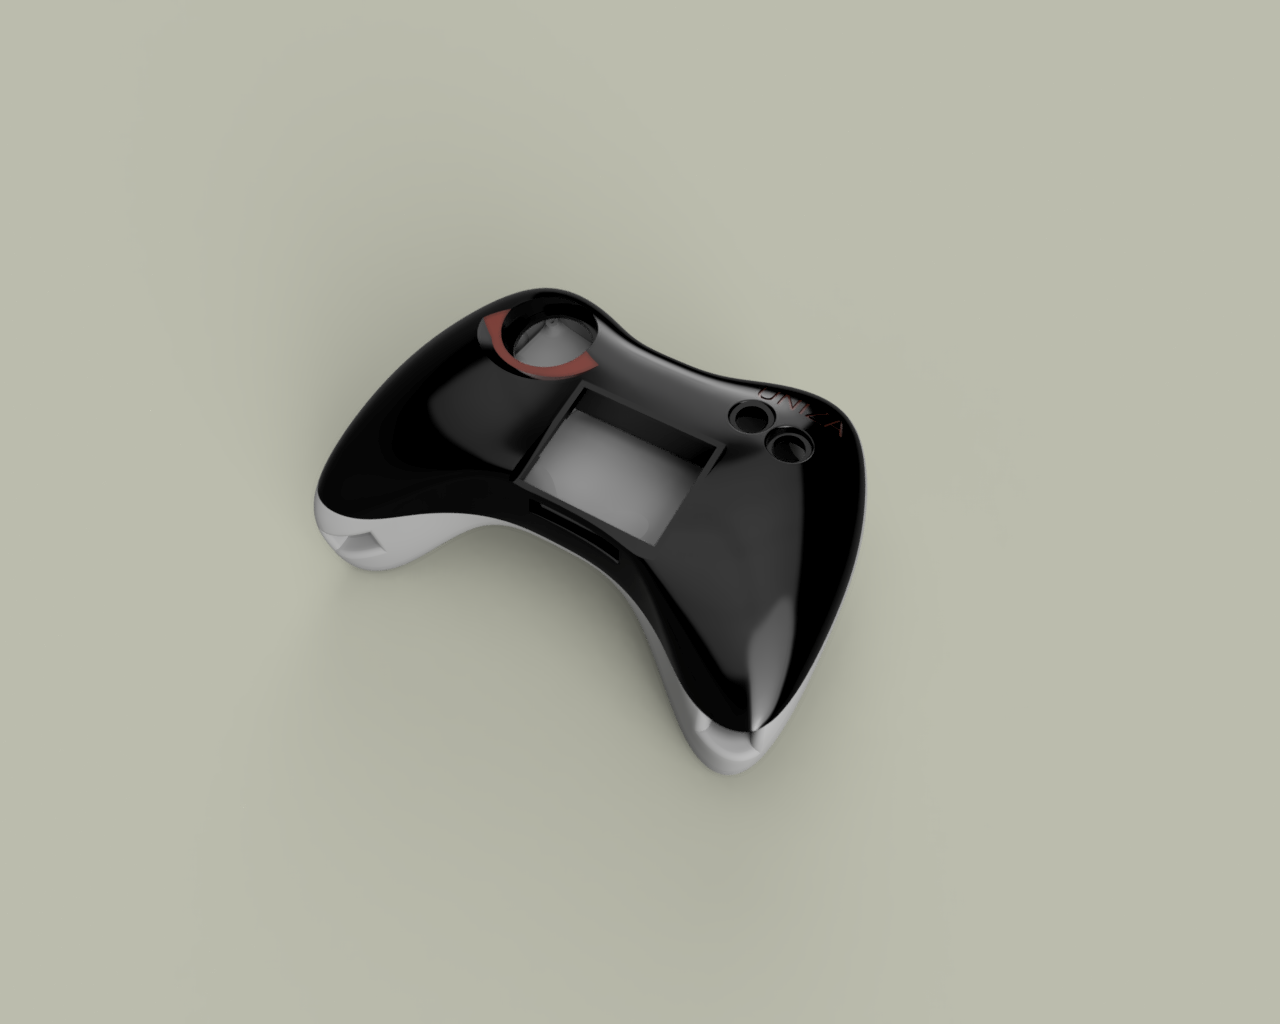
\includegraphics[width=8cm]{kontrolerVizu}
\caption{Ovládač balansujúceho robota}
\label{fig:kontrolerVizu}
\end{figure}

Napájanie ovládača je riešené z klasickej 9V batérie, zredukovanej spínaným zdrojom na $5V$ a na samotnú komunikáciu slúži modul HC-05 spomenutý v prvej časti tejto kapitoly. Okrem vysielania riadiacich príkazov ovládač v periodických intervaloch prijíma od robota dáta o jeho stave, ktoré následne zobrazuje užívateľovi na displeji.
 
Ovládač je schopný zobraziť informácie o uhle náklonu robota, aktuálnej rýchlosti, priemernej rýchlosti, aktuálnych kalibračných hodnotách a stave batérie. Používateľ môže taktiež prostredníctvom ovládača dať robotovi pokyn na začatie autokalibrácie a odoslanie dát do počítača cez sériový port.

Na rozdiel od predchádzajúceho prípadu, kedy sme navrhli okrem šasi taktiež dosku plošných spojov, v prípade ovládača neexistujú požiadavky na nijakú dodatočnú elektroniku a tak táto potreba odpadá. Komponenty budú spojené vnútri ovládača priamo s vývojovou doskou Arduino Nano. Malé rozmery tejto dosky zabezpečia, že rozmery ovládača budú podobné bežne predávaným konzolovým ovládačom. 

Ako problematická sa ukázala spotreba spínaného regulátora napätia, ktorá  bola v prípade nezaťaženého regulátora až $8 mA$. Takýto trvalý odber by nami použitú batériu rýchlo zničil, pristúpili sme teda k priradeniu spínača, ktorým bude batériu možné priamo odpojiť, keď bude ovládač nepoužívaný.

